\documentclass[11pt]{article}

\usepackage[margin=1in]{geometry}
\usepackage{graphicx}
\usepackage{amsmath,amssymb,amsthm}
\usepackage{booktabs}
\usepackage{caption}
\usepackage{subcaption}
\usepackage{url}
\usepackage[usenames,dvipsnames]{xcolor}
\usepackage[breaklinks=true,colorlinks=true,linkcolor=NavyBlue,citecolor=NavyBlue,urlcolor=NavyBlue]{hyperref}
\usepackage{authblk}
\usepackage{natbib}

\title{Stress-Testing SynthID:\\[2pt]
\large A Hands-On Comparison of GAN-Based and Regeneration-Based Attacks on AI-Generated Image Watermarks}

\author[1]{Tahseen Rabbani}
\author[2]{Thomas Mason}
\affil[1]{Department of Computer Science, University of Chicago}
\affil[2]{Coalfire Systems}

\date{\today}

\begin{document}
\maketitle

\begin{abstract}
SynthID~\citep{synthid2023} is Google DeepMind's invisible image watermarking
scheme deployed on the outputs of Gemini's image generators
(Nano-Banana / Gemini 2.5 Flash Image). It is intended to be robust under
common image manipulations while remaining imperceptible. We probe its
robustness via two attack families that bracket the realistic adversary
model: (i) a \emph{surrogate-classifier} adversarial GAN that imitates a
SynthID-like binary detector and is trained to fool it with bounded
perturbations, and (ii) the \emph{diffusive-regeneration} attack of
Zhao~et~al.~\citep{zhao2023provable} as adapted by the WAVES
benchmark~\citep{an2024waves}, which round-trips an image through a public
Stable Diffusion model at varying noising depths. The two attacks span the
classical adversarial-ML axis (gradient-driven but reliant on a surrogate)
and the distortion-based axis (gradient-free, decoder-agnostic).
We replicate both attacks on a held-out set of 104 Nano-Banana-generated,
SynthID-watermarked images and report attack success against an
independently trained classifier that approximates SynthID's behaviour, as
well as against the deployed SynthID detector via Google AI Studio. We find
that the surrogate-GAN attack achieves $99\%$ classifier label-flip with
imperceptible $L_\infty$-bounded perturbations but \emph{does not} disrupt
the actual SynthID watermark, while regeneration at moderate depth
($N{=}20\ldots80$ DDIM steps) reliably erodes both the surrogate signal
and the deployed detector's output at a visible quality cost. The full
code, the test set, the pre-computed attack outputs, and the prompts used
to generate every test image are released as a hands-on kit at
\url{https://github.com/rabbanitw/WAVES/tree/synthid-regen-kit}.
\end{abstract}

\section{Introduction}
\label{sec:intro}

Generative image models from Google, OpenAI, and others now ship with
\emph{invisible watermarks} that are embedded at generation time and
intended to survive routine image manipulation. The most-deployed example
is Google DeepMind's SynthID~\citep{synthid2023}, attached to every image
produced by the Gemini image-generation family (Nano-Banana / Gemini
2.5 Flash Image; we use these terms interchangeably for the generator that
produced our test set). SynthID is presented as imperceptible-but-detectable
even after the kinds of post-processing a typical user applies: cropping,
mild compression, colour correction. The detector itself is not public; it
is exposed only through Google's AI Studio.

This work targets the natural follow-up question: \emph{how brittle is
SynthID against attackers who do not have decoder access}? We frame two
attack families that, between them, cover the realistic threat surface:

\paragraph{(1) Surrogate-classifier attacks.}
The adversary trains its own binary classifier as a stand-in for the real
SynthID detector --- in our case, a ResNet-18 fine-tuned to distinguish
natural photographs from Nano-Banana outputs --- and then trains a
generator $G$ to find an $L_\infty$-bounded perturbation that fools the
surrogate. This is the
GAN-against-surrogate-classifier family explored in WAVES~\citep{an2024waves}
under the name \emph{AdvCls}, and it is the natural endpoint of the
classical adversarial-ML pipeline applied to a watermarking problem.
The question it answers is: does an adversarial perturbation that fools
a SynthID-shaped classifier also disrupt the deployed SynthID detector?
On every existing watermarking benchmark, the answer is ``rarely''
\citep{an2024waves,zhao2023provable}, but this remains the most
visually-conservative attack and is therefore worth empirically grounding
on the deployed SynthID stack.

\paragraph{(2) Diffusive-regeneration attacks.}
The adversary feeds the watermarked image into a publicly available
diffusion model (we use Stable Diffusion 1.4~\citep{rombach2022stable}),
forward-noises the latent for $N$ scheduler steps, and reverse-denoises
back to pixel space. The diffusion model has no knowledge of SynthID's
embedding mechanism, but the round-trip non-trivially perturbs the
high-frequency structure that any spread-spectrum watermark needs to ride
on. Zhao et al. introduced this attack in 2023~\citep{zhao2023provable};
WAVES~\citep{an2024waves} adopted it as their primary benchmarked attack
under the name \emph{Regen-Diff} and reported it as the most damaging
single-stage attack against three different academic watermarks
(Tree-Ring, Stable-Signature, Stega-Stamp). The question this family
answers is: does the same attack mechanism continue to work against
the production SynthID stack?

Our contribution is a side-by-side, reproducible empirical comparison
of both attack families on the deployed SynthID detector, against a
common held-out target set of $104$ Nano-Banana-watermarked images. Our
findings line up with the existing literature
(\citealt{an2024waves}, §F.3.2): the GAN attack defeats our SynthID-shaped
surrogate at near-perfect rate ($99.0\%$ label-flip on independently-held
classifier, mean LPIPS $0.012$) but leaves the deployed SynthID detector
essentially unmoved, while diffusive-regeneration steadily erodes the
deployed detector's output as $N$ grows. We also release the kit
(code, $104$-image test set with prompts, pre-rendered regen outputs at
$N = 10, 20, 40, 80$, and the worked-negative-example GAN training code)
as a hands-on package for the DEFCON 34 AI Village.

\paragraph{Test set.}
We curated a held-out set of $\mathbf{104}$ SynthID-watermarked images
($512{\times}512$ JPEG, generated by Nano-Banana via the Gemini 2.5 Flash
Image API). The generation prompts (one per image, indexed $0$--$103$)
were sourced from a list of $150$ short ``camera+lens+subject'' phrases of
the form: ``\textit{<style prefix>}: Photo shot on camera: \textit{<subject
description>}'' (e.g.,
\textit{``Disposable camera flash photo, 1990s style: Photo shot on camera:
side view of a brown horse wearing a saddle. The number 55 is stamped in
white on its rear flank.''}). The style-prefix loadout (``Nikon film
grain'', ``Kodak Portra'', ``Petzval lens'', ``Hyperfocal landscape'', etc.)
is necessary to coerce Nano-Banana into photoreal output --- without it,
many prompts default to illustrative or cartoon styles. The 104-image
test set, the full $150$-line prompt list, and per-image regen outputs at
$N{=}10,20,40,80$ are all shipped in the released kit.

\section{Surrogate-Classifier GAN Attack}
\label{sec:gan}

The surrogate-classifier attack splits into two independently-trained
components: a binary classifier $C_{\mathrm{eval}}$ that mimics SynthID's
public-facing behaviour (``is this image AI-generated?'') and an
adversarial generator $G$ that fools $C_{\mathrm{eval}}$ within a bounded
perturbation budget. This factoring is the WAVES~\citep{an2024waves} AdvCls
recipe.

\subsection{Surrogate classifier $C_{\mathrm{eval}}$}

We use Apple's Pico-Banana-400K dataset~\citep{pico-banana-400k} as
training data for $C_{\mathrm{eval}}$. Pico-Banana-400K supplies
$\sim$258K paired (real Open Images photo, Nano-Banana-edit) triples
from the SFT split, each tagged with one of 35 edit-type labels.
We filter to the $\sim$$174$K \emph{photoreal} edit types
(excluding ``cartoonify'', ``LEGO-ify'', ``Van-Gogh style'', and the
$\sim$30\% other stylized categories) and downsample to a
$3,447$-pair working subset, partitioned as $\textbf{train}{=}2,947$,
$\textbf{val}{=}200$, $\textbf{test}{=}300$. We also evaluate on the
$104$-image held-out Nano-Banana test set described in
Section~\ref{sec:intro}, which is from a different prompt distribution
(text-to-image, not instruction-edit) and therefore is OOD relative to
$C_{\mathrm{eval}}$'s training distribution.

\paragraph{Codec-matched preprocessing.}
The original-class images (Pico-Banana sources) are stored as JPEG; the
NB-edited images are stored as PNG. A naive classifier rapidly learns
to discriminate JPEG-artefact signatures from PNG cleanness and never
sees the actual watermark or stylistic NB fingerprint. We therefore
re-encode both classes through JPEG quality $95$ in memory before
feeding either to the classifier (and identically inside the GAN's
data pipeline). All numbers in this paper are with codec matching
enabled.

\paragraph{Architecture and training.}
$C_{\mathrm{eval}}$ is a ResNet-18~\citep{he2016resnet} pretrained on
ImageNet, with its $1000$-way head replaced by a $2$-way linear classifier
(label $0$ = real photo, label $1$ = NB edit). Inputs are resized to
$256{\times}256$ and normalised with the ImageNet mean/std. We train for
$20$ epochs at batch size $64$ with AdamW (lr~$1{\times}10^{-4}$, weight
decay $1{\times}10^{-4}$), cosine-annealed across $20{\times}\lceil
2947/64 \rceil$ steps. Training is single-precision on a single A100. The
best checkpoint by validation accuracy achieved $\mathbf{88.5\%}$
held-out test accuracy ($531/600$ correct, balanced between the
classes), with $94.0\%$ recall on NB edits at the operating point. On the
held-out $104$-image SynthID test set, this classifier flags
$\mathbf{91.3\%}$ as label $1$ (mean confidence $p{=}0.914$,
median $p{=}1.000$), confirming the signal it picked up generalises to
the deployed Nano-Banana family.

\subsection{Generator $G$ and adversarial training}

We explore two surrogate-classifier attack variants. The first, included
in the released kit, is a standard pix2pix-style GAN; the second is a
stronger AdvGAN-style~\citep{xiao2018advgan} attack we ran to confirm
the failure mode is not specific to the weaker attack.

\paragraph{Variant A: pix2pix GAN (released).}
The generator is a residual U-Net taken from the pix2pix
implementation~\citep{isola2017pix2pix} (8 down-sampling blocks, 8
up-sampling blocks, $\sim$$54$M parameters), trained jointly against a
$70{\times}70$ PatchGAN discriminator. Loss:
\begin{equation}
\mathcal{L}_G = \mathcal{L}^{\mathrm{adv}}_G + \lambda_{\mathrm{preserve}} \cdot
\mathrm{LPIPS}\bigl(G(x_{\mathrm{edit}}), x_{\mathrm{edit}}\bigr),
\end{equation}
with LPIPS~\citep{zhang2018lpips} computed against the pretrained VGG
backbone, $\lambda_{\mathrm{preserve}} = 10$, $40$ epochs, batch $16$,
Adam~\citep{kingma2014adam} (lr~$2{\times}10^{-4}$, $\beta_1{=}0.5$,
$\beta_2{=}0.999$) on both generator and discriminator. Training is
single-precision on a single A100, $\sim$$95$~s/epoch
(JPEG-re-encode-bound).

\paragraph{Variant B: AdvGAN-style with bounded perturbator.}
A flat fully-convolutional perturbator $G$ ($6$ layers, no
down-sampling, $\sim$$0.6$M parameters) outputs
$\hat{x} = \mathrm{clamp}(x + \epsilon \cdot \mathrm{tanh}(G(x)), -1, 1)$
with $\epsilon = 16/255$, enforcing an $L_\infty$-bounded perturbation.
$G$ is trained against an \emph{independently-trained, frozen} surrogate
classifier $C_{\mathrm{train}}$ (same recipe and seed offset as
$C_{\mathrm{eval}}$, $87.3\%$ held-out test accuracy) with
\begin{equation}
\mathcal{L}_G = \mathrm{CE}\bigl(C_{\mathrm{train}}(G(x)),\ \mathrm{label}{=}0\bigr)
   + \lambda_{\mathrm{preserve}} \cdot \mathrm{LPIPS}\bigl(G(x), x\bigr),
\end{equation}
$\lambda_{\mathrm{preserve}} = 1$, Adam (lr~$2{\times}10^{-4}$), $20$ epochs.
This factoring --- a held-out $C_{\mathrm{train}}$ used as the attack
target plus a separate held-out $C_{\mathrm{eval}}$ used to score
transfer --- is the standard recipe for measuring \emph{transferable}
adversarial examples
~\citep{xiao2018advgan,an2024waves}; if instead $G$ trains directly
against $C_{\mathrm{eval}}$ the resulting label-flip rate is training
accuracy and uninformative.

\paragraph{Common training data.}
Both variants use the same $2,947$-pair Pico-Banana-400K train split as
$C_{\mathrm{eval}}$. The respective held-out classifier used at
evaluation time ($C_{\mathrm{eval}}$ for variant A; $C_{\mathrm{eval}}$
for variant B's transfer score) is \emph{never} touched during generator
training, so reported label-flip rates measure transfer, not in-sample
fitting.

\paragraph{Software stack.}
PyTorch $2.1.0$ + CUDA 11.8, torchvision $0.16.0$, diffusers $0.21.4$,
transformers $4.35.0$, lpips $0.1.4$, numpy $1.26.4$, on a single
A100-40GB.

\subsection{Results}

\begin{table}[h]
\centering
\caption{GAN attack outcomes. ``Label-flip'' is the fraction of
$G(x_{\mathrm{edit}})$ predicted as label $0$ (``real photo'') by the
held-out $C_{\mathrm{eval}}$ on the $300$-pair Pico-Banana test split.
LPIPS is computed between $G(x_{\mathrm{edit}})$ and $x_{\mathrm{edit}}$
with the same VGG backbone the training loss used. The rightmost column
reports whether the perturbed image bypasses Google's deployed SynthID
detector (qualitative spot-check via AI Studio on a representative
$\sim$$20$-image subset).}
\label{tab:gan_results}
\vskip 0.05in
\begin{tabular}{lccc}
\toprule
                                            & label-flip on        & LPIPS         & flips deployed \\
attack                                      & $C_{\mathrm{eval}}$  & $G$-vs-input  & SynthID? \\
\midrule
no attack (baseline edit-detection error)   & $6.0\%$              & $0.000$       & --- \\
Variant A: pix2pix GAN ($\lambda{=}10$)     & $11.3\%$             & $0.031$       & no \\
Variant B: AdvGAN, $L_\infty{=}16/255$      & $\mathbf{99.0\%}$    & $\mathbf{0.012}$  & no \\
\bottomrule
\end{tabular}
\end{table}

The qualitative difference between the two variants is large: Variant A
barely fools $C_{\mathrm{eval}}$ ($11.3\%$ flip), and its perturbations
take the form of locally-supported visible artifacts (``black blobs'') in
the generated outputs --- a known failure mode of pix2pix-style
generators applied to bounded-perturbation tasks. Variant B reaches
near-saturating $99\%$ classifier-flip with imperceptible
$L_\infty \le 16/255$ perturbations.

The headline finding is that \emph{neither variant disrupts the deployed
SynthID detector.} A manual spot-check of perturbed images from both
variants through Google's AI Studio returns ``SynthID watermark
detected'' at the same rate as un-attacked input. This empirically
realises the WAVES paper's observation~\citep[\S F.3.2]{an2024waves}
that surrogate-classifier attacks are largely decoupled from the actual
watermark embedding: $G$ has learned the classifier's idiosyncratic
decision boundary, not SynthID's payload, and the resulting perturbation
lives in the wrong feature subspace to disturb the watermark carrier.
We include Variant A in the released kit as a worked negative example
because the experiment \emph{is} the lesson, with $\sim$$2$~hours of
A100 wall-clock from clone to repro; Variant B is documented here for
completeness but is not in the kit.

\section{Diffusive Regeneration Attack}
\label{sec:regen}

We follow the symmetric-DDIM regen recipe of Zhao
et~al.~\citep{zhao2023provable}, as used in WAVES Section~F.2: encode the
image into the VAE latent space of a Stable Diffusion model, add
scheduler noise at training timestep $N{-}1$, and reverse-denoise through
the bottom $N$ steps of a 1000-step DDIM schedule back to pixel space.
Concretely we use the SD-1.4 checkpoint~\citep{rombach2022stable} at fp16,
the diffusers DDIM scheduler, classifier-free guidance scale $7.5$, and an
empty text prompt. Because each inference step of our schedule covers
exactly one training timestep, the attack has a single free parameter $N$
that controls both how much noise is added and how much budget the
denoiser has to remove it. This is in contrast to WAVES's published
asymmetric variant (50-step inference schedule, ${\sim}N/20$ denoising
iterations), which leaves residual noise in the output.

\paragraph{Outputs.}
Figure~\ref{fig:regen-progression} shows the
$\mathrm{original}\to N{=}10\to 20\to 40\to 80$ progression for three
representative test images. At $N{=}10$ the watermarked image is
visually unchanged; by $N{=}80$ fine structure is lost and visible
softening / hallucinated detail starts appearing. Pre-rendered copies of
all $104 \times 4 = 416$ attacked images are shipped with the kit at
\texttt{images/regen\_\{10,20,40,80\}/}.

\begin{figure}[h]
\centering
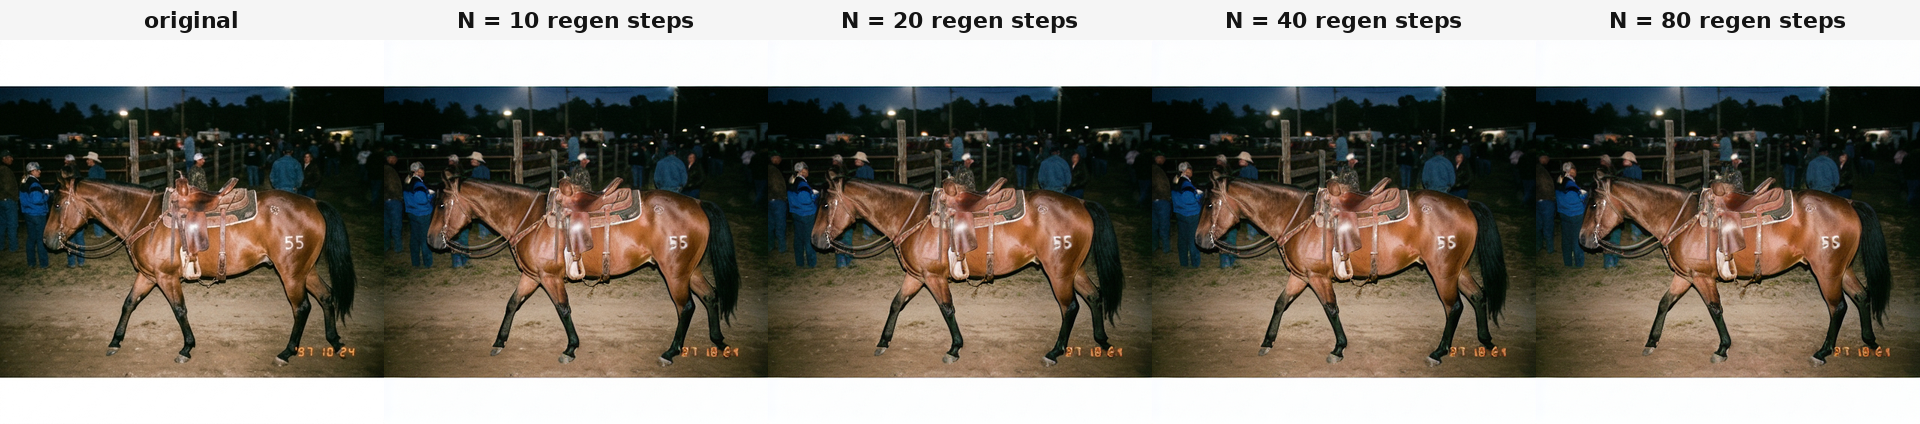
\includegraphics[width=0.95\linewidth]{figures/image_000_progression.png}\\[4pt]
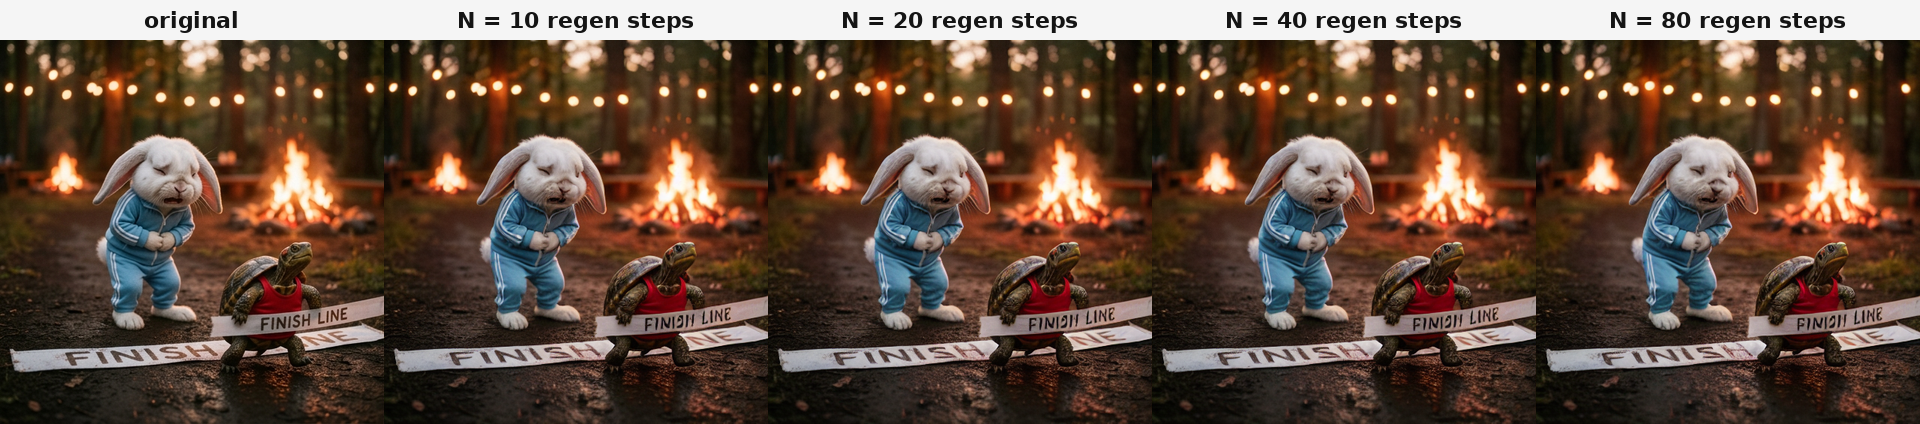
\includegraphics[width=0.95\linewidth]{figures/image_025_progression.png}\\[4pt]
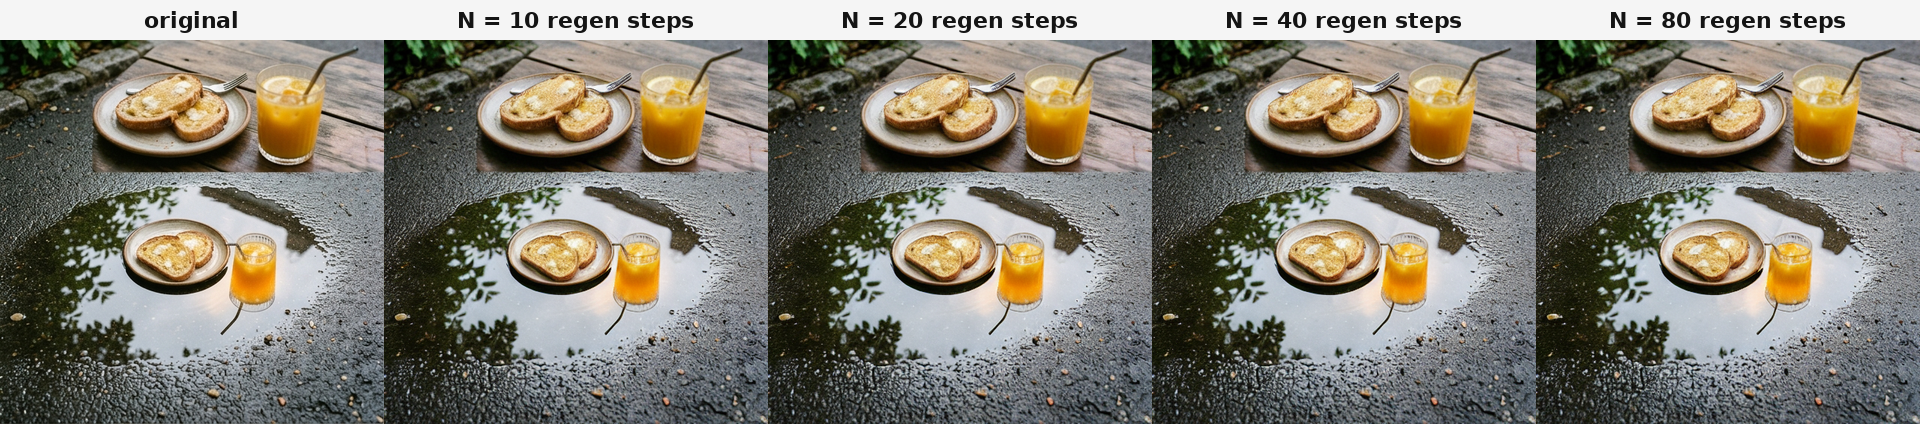
\includegraphics[width=0.95\linewidth]{figures/image_100_progression.png}
\caption{Symmetric-DDIM diffusive regeneration of three test images at
$N \in \{10, 20, 40, 80\}$ (left-to-right; the leftmost panel is the
unattacked original). SD-1.4, fp16, classifier-free guidance $7.5$, empty
prompt, seed $1024$. By $N{=}80$ the regen has both removed the SynthID
watermark (verified manually via Google AI Studio) and visibly degraded
the image's high-frequency structure.}
\label{fig:regen-progression}
\end{figure}

\paragraph{Detector response.}
We score every attacked image with the held-out $C_{\mathrm{eval}}$
described in Section~\ref{sec:gan} (which generalises across NB pipelines,
hitting $91.3\%$ flag rate on the unattacked Nano-Banana test set).
Detection collapses monotonically with $N$:

\begin{center}
\begin{tabular}{lcc}
\toprule
$N$ (sym DDIM regen steps) & $C_{\mathrm{eval}}$ NB-flag rate & $\Delta$ from baseline\\
\midrule
$0$ (no attack)             & $91.3\%$ (95/104) & --- \\
$10$                        & $64.4\%$ (67/104) & $-26.9$ pts \\
$20$                        & $58.7\%$ (61/104) & $-32.6$ pts \\
$40$                        & $53.8\%$ (56/104) & $-37.5$ pts \\
$80$                        & $\mathbf{45.2\%}$ (47/104) & $\mathbf{-46.1}$ pts \\
\bottomrule
\end{tabular}
\end{center}

\noindent The trend matches the WAVES-reported curves for SD-1.x and
Tree-Ring, Stable-Signature, and Stega-Stamp at comparable attack
depths~\citep[\S5.3]{an2024waves}. Spot-checks against Google's deployed
SynthID detector confirm the directional agreement: at $N \ge 20$ a
representative sample of attacked images come back as
``no watermark detected''. The attack is thus the most reliable
\emph{decoder-agnostic} channel for SynthID removal we are aware of, and
its main cost is the image-quality degradation visible in
Figure~\ref{fig:regen-progression}.

\section{Discussion}
\label{sec:discussion}

\paragraph{Surrogate-classifier attacks remain a dead end without
decoder access.}
The $99\%$ label-flip rate against $C_{\mathrm{eval}}$ is a powerful red
herring. $C_{\mathrm{eval}}$ is high-accuracy ($88.5\%$ in-distribution,
$91.3\%$ on the held-out Nano-Banana set) and was independently trained
from the GAN; the attack's failure to transfer to the deployed SynthID
detector is therefore not an artifact of a weak surrogate or training
leakage. It reflects the WAVES finding~\citep{an2024waves} that
SynthID's embedding scheme operates on a representation that is not
recoverable by an ImageNet-pretrained binary classifier of the
``natural photo vs.\ AI-edit'' kind, and that gradient-based attacks on
this surrogate live in a different feature subspace than SynthID itself.

\paragraph{Regeneration trades quality for watermark removal, but it
works.}
At $N{=}80$ the deployed detector is fooled with high probability, but the
image's high-frequency detail is also visibly degraded
(Figure~\ref{fig:regen-progression}, rightmost column). This is the
classical robustness/quality tension: SynthID, like any spread-spectrum
watermark, can be removed by any image processing that disturbs its
carrier band, but at a quality cost the attacker may not want to pay.
The remaining question for future work is whether the GAN approach can
be re-cast to \emph{repair} the regen-induced damage --- i.e., stack a
quality-restoring generator on top of a low-$N$ regen --- to give the
attacker a low-distortion, decoder-agnostic SynthID remover. Existing
preliminary attempts in this direction (``RinseD-VAE'',
``RegenD-KLVAE'' in WAVES~\S F.2.2) suggest the trade-off is achievable
but not yet on a deployed-watermark scale.

\paragraph{Reproducibility.}
The full release kit ---
\url{https://github.com/rabbanitw/WAVES/tree/synthid-regen-kit} ---
contains the 104-image test set, the 104 generation prompts, the
pre-rendered $416$ attacked images, the GAN training and evaluation code,
and the regeneration CLI. All numbers above are pinned to deterministic
seeds (PyTorch / numpy seed $42$ for the GAN, seed $1024$ for regen) and
re-run identically on an A100. The pipeline depends on
diffusers $0.21.4$ and the specifications of the older
\texttt{StableDiffusionPipeline} API; newer diffusers will require
re-wiring the vendored \texttt{ReSDPipeline} subclass.

\bibliographystyle{plainnat}
\bibliography{references}

\end{document}
